% Entrega 2: reporte técnico de avance (mismo formato de la Entrega 1).
% Compilar con: xelatex informe_avance.tex (dos veces)
\documentclass[11pt,a4paper]{article}
\usepackage[top=2.1cm,bottom=2.0cm,left=2.0cm,right=2.0cm,headsep=0.6cm]{geometry}
\usepackage{fontspec}
\setmainfont{Liberation Serif}
\usepackage{babel}
\babelprovide[import,main]{spanish}
\usepackage{microtype}
\usepackage{tabularx,array,booktabs}
\usepackage{enumitem}
\usepackage{titlesec}
\usepackage{caption}
\usepackage{graphicx}
\usepackage{fancyhdr}
\usepackage[hidelinks]{hyperref}
\urlstyle{rm}

\AtBeginDocument{\renewcommand{\tablename}{Tabla}\renewcommand{\figurename}{Figura}}
\linespread{1.0}
\setlength{\parskip}{2pt}
\setlength{\parindent}{1.2em}
\titleformat{\section}{\large\bfseries}{\thesection.}{0.5em}{}
\titlespacing*{\section}{0pt}{8pt}{3pt}
\setlist{itemsep=1pt,topsep=3pt,parsep=0pt,leftmargin=1.5em}
\captionsetup{font=small,labelfont=bf,labelsep=period,skip=4pt,justification=justified,singlelinecheck=false}
\setlength{\textfloatsep}{9pt plus 2pt minus 2pt}
\setlength{\floatsep}{8pt plus 2pt minus 2pt}
\setlength{\intextsep}{8pt plus 2pt minus 2pt}
\newcommand{\code}[1]{\textit{#1}}
\newcolumntype{Y}{>{\raggedright\arraybackslash}X}
\setlength{\emergencystretch}{2em}

\pagestyle{fancy}
\fancyhf{}
\fancyhead[L]{\small\textit{Técnicas Avanzadas de Modelado · Entrega 2}}
\fancyhead[R]{\small\textit{Reconocimiento de señas aisladas LSC-54}}
\fancyfoot[C]{\small\thepage}
\renewcommand{\headrulewidth}{0.4pt}
\fancypagestyle{plain}{\fancyhf{}\fancyfoot[C]{\small\thepage}\renewcommand{\headrulewidth}{0pt}}

\begin{document}

\thispagestyle{plain}
\begin{center}
{\Large\bfseries Reconocimiento de señas aisladas de la Lengua de Señas Colombiana:\\[3pt] una red recurrente sobre landmarks frente a una línea base clásica}\\[8pt]
{\normalsize Andrés Díaz, Lorena Valero, Jorge Anaya y Sabrina Miranda}\\[3pt]
{\small Maestría en Analítica Aplicada e Inteligencia Artificial, Universidad de La Sabana}\\
{\small Técnicas Avanzadas de Modelado, 2026-II \,·\, Entrega 2: reporte técnico de avance \,·\, Octubre de 2026}\\[2pt]
{\small\url{https://github.com/andresdila/lsc54-reconocimiento-senas}}
\end{center}
\vspace{2pt}
\noindent\rule{\textwidth}{0.4pt}
\vspace{0pt}

%--------------------------------------------------------------------------------------
\section{Problema, datos y diseño experimental}

El proyecto busca reconocer 43 señas aisladas de la Lengua de Señas Colombiana (LSC) con la campaña S2 del conjunto LSC-54 (Mora-Zarate et al., 2025): 33 expresiones de cortesía y los números del uno al diez, grabados por 18 señantes en 1.740 videos. El uso previsto es una herramienta de práctica en la que un estudiante hace la seña frente a la cámara y el sistema indica si corresponde a la solicitada; por ello, la pregunta relevante es qué tan bien reconoce el modelo a una persona que nunca ha visto, y toda la evaluación se hace por señante y no por video.

Cada video pasa por MediaPipe Holistic (Lugaresi et al., 2019) y se convierte en una serie de 98 coordenadas por cuadro: siete puntos del tren superior y los 21 de cada mano, en píxeles y normalizados por el ancho de hombros. En la Entrega 1, cada serie se resumió en 493 estadísticas para una regresión logística, con macro-F1 de 0,549 en validación cruzada. En esta entrega se implementa en PyTorch la red propuesta en el plan, una BiGRU con atención temporal que lee la secuencia completa, y se compara con esa línea base en las mismas condiciones (Tabla~\ref{tab:protocolo}), bajo la hipótesis de que el orden y la dinámica del movimiento contienen información que los resúmenes estadísticos pierden.

Frente al plan se introduce un cambio: en lugar de parada temprana sobre el fold de validación, cada modelo se entrena 80 épocas fijas y se reporta la métrica de la última. Con dos señantes por fold, escoger la mejor época con ese mismo fold infla la estimación; en el modelo base, la mejor época supera a la última en 0,019 de macro-F1 en promedio, que es el sesgo que se habría introducido.

\begin{table}[htbp]
\centering
\caption{Protocolo experimental, común a la línea base y a todos los experimentos.}\label{tab:protocolo}
\small
\renewcommand{\arraystretch}{1.1}
\begin{tabularx}{\textwidth}{@{}>{\raggedright\arraybackslash}p{3.4cm}Y@{}}
\toprule
\textbf{Elemento} & \textbf{Valor}\\
\midrule
Datos & LSC-54, campaña S2: 1.740 videos, 43 clases, 18 señantes; MediaPipe 0.10.21, 98 coordenadas por cuadro\\
Partición v1 (Entrega 1) & Desarrollo: 14 señantes en 7 folds de 2 personas (1 \emph{full} y 1 \emph{partial}). Test bloqueado: 4 señantes (381 videos), evaluado una sola vez al final\\
Métrica y regla de decisión & Macro-F1. El modelo avanzado gana si mejora en al menos 0,05 y en al menos 5 de 7 folds; la diferencia se acompaña de un IC del 95\,\% por remuestreo de señantes\\
Entrenamiento & Entropía cruzada, AdamW, lotes de 32, 80 épocas fijas, calentamiento lineal de 5 épocas y decaimiento coseno, recorte del gradiente en 1,0\\
Control y entorno & Un factor por experimento; mismos folds y semilla (2026 más el fold); registro en MLflow y JSON/CSV con commit. Windows, CPU; Python 3.11, PyTorch 2.14.1, scikit-learn 1.9.1\\
\bottomrule
\end{tabularx}
\end{table}

%--------------------------------------------------------------------------------------
\section{Preparación de las secuencias y de los tensores}

Dos características de los datos condicionan el preprocesamiento (Figura~\ref{fig:datos}). La primera es la duración: los videos van de 16 a 335 cuadros, con mediana de 53 y dos grupos, alrededor de 40 y de 90 cuadros, que probablemente corresponden a señas cortas y a señas con más de un movimiento. La segunda es la detección: MediaPipe encuentra la pose en el 99,5\,\% de los cuadros, pero la mano más activa solo en el 60\,\%, con tasas por persona de 0,46 a 0,97; además, los señantes del test tienen mejor detección que los de desarrollo (0,73 frente a 0,57).

\begin{figure}[htbp]
\centering
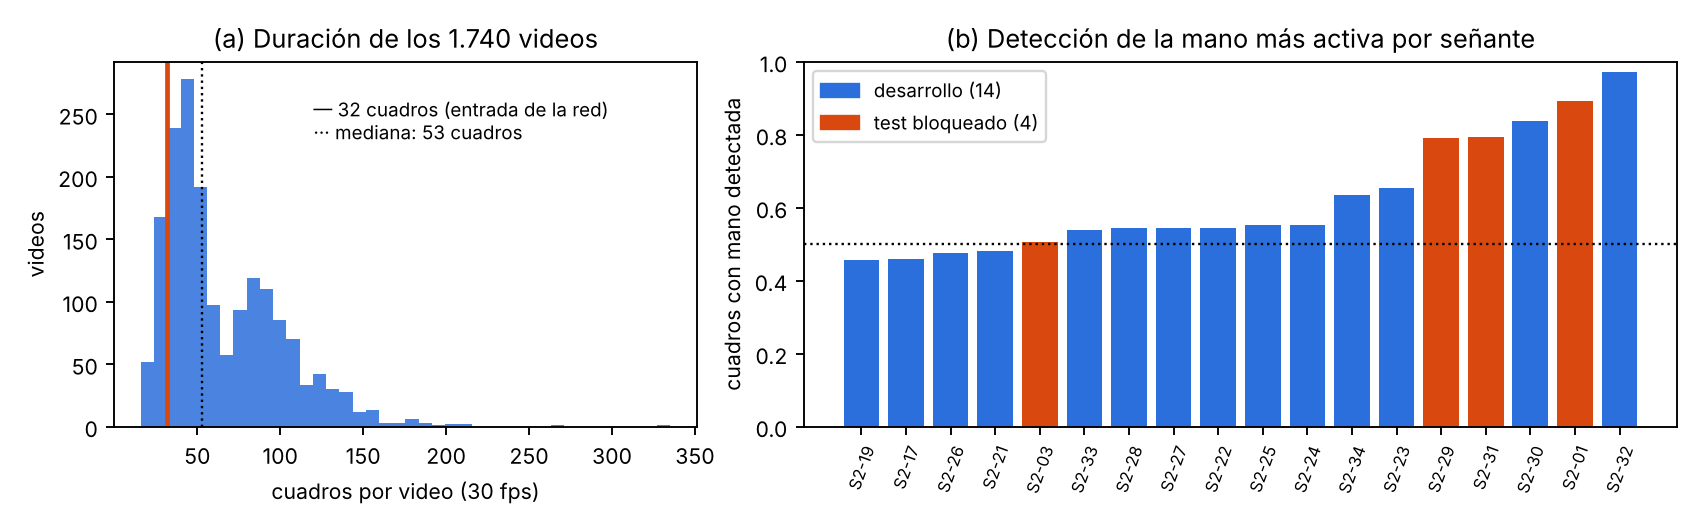
\includegraphics[width=0.68\textwidth]{figures/fig1_datos.png}
\caption{(a) Cuadros por video, con la longitud de entrada (32) y la mediana (53); (b) detección de la mano más activa por señante (naranja: test).}\label{fig:datos}
\end{figure}

Cada secuencia pasa por los pasos de la Tabla~\ref{tab:prepro}. Solo la estandarización aprende de los datos, y se ajusta en cada fold con los señantes de entrenamiento, de modo que la validación nunca entra al preprocesamiento. El resultado es un tensor de $32 \times 101$ por video (98 coordenadas y 3 canales de máscara), con lotes de $32 \times 32 \times 101$; junto a cada video viaja el logaritmo estandarizado de su duración, porque el remuestreo la elimina.

\begin{table}[htbp]
\centering
\caption{Pasos del preprocesamiento secuencial (\code{src/lsc/features/sequence.py}).}\label{tab:prepro}
\small
\renewcommand{\arraystretch}{1.1}
\begin{tabularx}{\textwidth}{@{}>{\raggedright\arraybackslash}p{2.8cm}>{\raggedright\arraybackslash}p{5.0cm}Y@{}}
\toprule
\textbf{Paso} & \textbf{Parámetro} & \textbf{Justificación}\\
\midrule
Filtro de plausibilidad & Cuadros con algún punto a más de 6 anchos de hombro pasan a ausentes & Si los hombros se estiman casi superpuestos, la escala colapsa y las coordenadas se disparan\\
Relleno de vacíos cortos & Interpolación lineal de vacíos de hasta 5 cuadros ($\approx$\,0,17 s), solo si hay detección a ambos lados & Una mano que desaparece un instante no cambia la seña; no se extrapola al inicio ni al final\\
Remuestreo & 32 cuadros equiespaciados, vecino más cercano & Longitud fija para formar lotes sin inventar posiciones intermedias\\
Máscara de detección & 3 canales binarios (pose, mano izquierda y mano derecha); lo ausente pasa a 0 & Distingue una mano ubicada en el origen de una mano que no se detectó\\
Estandarización & Media y desviación por coordenada, solo con el entrenamiento del fold & Evita la fuga de información y unifica escalas\\
Aumentación (solo entrenamiento) & Recorte temporal hasta 10\,\% por extremo, escala $\pm$10\,\%, rotación $\pm$10°, ruido $\sigma$\,=\,0,01 & Simula ritmo, distancia, postura y ruido de detección; sin reflejo horizontal, que cambia la mano dominante\\
\bottomrule
\end{tabularx}
\end{table}

La aumentación se sortea en cada época; validación y test usan la versión determinista. Las 22 pruebas automáticas del repositorio verifican, entre otras reglas, que la interpolación no rellena vacíos largos ni bordes, que la máscara coincide con la ausencia y que la aumentación es reproducible con la misma semilla.

%--------------------------------------------------------------------------------------
\section{Arquitectura de la red}

La red (\code{src/lsc/models/sequence.py}) sigue el flujo video $\rightarrow$ MediaPipe $\rightarrow$ secuencia $\rightarrow$ proyección $\rightarrow$ BiGRU $\rightarrow$ atención temporal $\rightarrow$ salida (Tabla~\ref{tab:capas}). Sus 552.023 parámetros son unas 26 veces los de la regresión logística (21.242), aunque pocos para una red recurrente entrenada con 1.359 videos.

\begin{table}[htbp]
\centering
\caption{Capas de la BiGRU base, dimensión de salida por video y número de parámetros.}\label{tab:capas}
\small
\renewcommand{\arraystretch}{1.1}
\begin{tabularx}{\textwidth}{@{}>{\raggedright\arraybackslash}p{4.6cm}>{\raggedright\arraybackslash}p{1.5cm}>{\raggedleft\arraybackslash}p{1.75cm}Y@{}}
\toprule
\textbf{Capa} & \textbf{Salida} & \textbf{Parámetros} & \textbf{Justificación}\\
\midrule
Entrada & $32 \times 101$ & --- & 98 coordenadas estandarizadas y 3 canales de máscara por cuadro\\
Proyección: lineal, LayerNorm, GELU y dropout 0,1 & $32 \times 128$ & 13.312 & Espacio común para coordenadas y máscara; LayerNorm controla colas largas\\
BiGRU, capa 1 (128 unidades por dirección) & $32 \times 256$ & 198.144 & Lee la secuencia en ambos sentidos\\
BiGRU, capa 2 (dropout 0,1 entre capas) & $32 \times 256$ & 296.448 & Combina patrones de corta duración en movimientos completos\\
Atención temporal: lineal 256$\rightarrow$128, tanh, lineal 128$\rightarrow$1, softmax & 256 & 33.025 & Un peso por cuadro en lugar de un promedio uniforme\\
Cabeza: dropout 0,3, log de la duración y lineal 257$\rightarrow$43 & 43 & 11.094 & Probabilidades de las 43 señas\\
\midrule
\textbf{Total} & & \textbf{552.023} & \\
\bottomrule
\end{tabularx}
\end{table}

Se prefiere la GRU (Cho et al., 2014) a la LSTM (Hochreiter y Schmidhuber, 1997) porque cumple la misma función con cerca de un 25\,\% menos de parámetros (la LSTM equivalente tiene 716.887), algo relevante con pocos datos. La bidireccionalidad es válida porque la seña se clasifica una vez termina el video, aunque no lo sería en traducción en línea. La atención responde a que, al inicio y al final de muchos videos, las manos están en reposo y se detectan mal, de modo que un promedio uniforme mezclaría esos cuadros con el núcleo de la seña. Usar landmarks, y no píxeles, reduce el costo y la sensibilidad al fondo, y evita usar el rostro.

Como verificación inicial, la pérdida de entrenamiento al cerrar la primera época es 3,68, cerca de $\ln 43 \approx 3{,}76$, lo esperado para un clasificador que aún no prefiere ninguna clase; después baja de forma continua en todos los folds, sin saltos ni valores no numéricos.

%--------------------------------------------------------------------------------------
\section{Entrenamiento y ajuste de hiperparámetros}

Se minimiza la entropía cruzada con AdamW (Loshchilov y Hutter, 2019), tasa de $10^{-3}$, weight decay de 0,01 (sin aplicarlo a sesgos ni a normalizaciones) y lotes de 32. La tasa sube de forma lineal en las cinco primeras épocas, para no dar pasos grandes con la red aún desordenada, y luego baja con una curva coseno hasta cero; el gradiente se recorta en 1,0, una precaución estándar en redes recurrentes, y cada fold se entrena desde cero.

El ajuste cambia un factor a la vez (Google Developers, s.~f.): cada experimento modifica un solo elemento de la configuración base, de modo que la diferencia se atribuye a ese elemento. Se corren 14 experimentos, unos de ajuste (tasa, regularización y optimizador) y otros de ablación, que quitan o cambian una pieza para saber si aporta. Todos usan los mismos folds, semilla y código (commit \code{dbbe611}), y cada corrida queda en MLflow (MLflow Project, s.~f.) y en \code{reports/e2\_avance/runs/} con configuración, métricas por fold, curvas y predicciones por video. El intervalo de cada diferencia frente a la base se obtiene remuestreando señantes con reemplazo 1.000 veces, la misma unidad de la partición (Tabla~\ref{tab:experimentos}).

\begin{table}[htbp]
\centering
\caption{Experimentos en validación cruzada por señante. Macro-F1 como media $\pm$ desviación estándar de los 7 folds; $\Delta$ es la diferencia de macro-F1 agrupado frente a la BiGRU base.}\label{tab:experimentos}
\small
\renewcommand{\arraystretch}{1.12}
\begin{tabularx}{\textwidth}{@{}lYcccc@{}}
\toprule
\textbf{Experimento} & \textbf{Cambio respecto a la base} & \textbf{Macro-F1} & \textbf{$\Delta$ vs. base} & \textbf{IC 95\,\% de $\Delta$} & \textbf{Top-3}\\
\midrule
Regresión logística$^{\ast}$ & Línea base de la Entrega 1 & 0,548 $\pm$ 0,166 & --- & --- & 0,783\\
\textbf{BiGRU base} & --- & \textbf{0,811 $\pm$ 0,079} & --- & --- & \textbf{0,923}\\
\midrule
conv1d & Conv1D en vez de GRU & 0,828 $\pm$ 0,066 & +0,019 & [$-$0,011; +0,044] & 0,934\\
wd0.1 & Weight decay 0,01 $\rightarrow$ 0,1 & 0,819 $\pm$ 0,073 & +0,006 & [$-$0,005; +0,020] & 0,940\\
sin\_interpolacion & No se rellenan vacíos cortos & 0,819 $\pm$ 0,065 & +0,005 & [$-$0,008; +0,019] & 0,937\\
pesos\_clase & Pérdida ponderada por clase & 0,810 $\pm$ 0,077 & $-$0,002 & [$-$0,013; +0,010] & 0,933\\
dropout0.5 & Dropout de la cabeza 0,3 $\rightarrow$ 0,5 & 0,805 $\pm$ 0,081 & $-$0,006 & [$-$0,023; +0,010] & 0,935\\
lr3e-3 & Tasa $10^{-3} \rightarrow 3\times10^{-3}$ & 0,801 $\pm$ 0,081 & $-$0,014 & [$-$0,029; +0,007] & 0,930\\
\midrule
sin\_mascara & Sin canales de detección & 0,794 $\pm$ 0,082 & $-$0,016 & [$-$0,033; $-$0,001] & 0,925\\
sin\_ncuadros & Sin la duración del video & 0,791 $\pm$ 0,089 & $-$0,020 & [$-$0,038; $-$0,003] & 0,936\\
sin\_aumentos & Sin aumentación & 0,771 $\pm$ 0,095 & $-$0,040 & [$-$0,077; $-$0,014] & 0,905\\
lstm & LSTM en vez de GRU & 0,754 $\pm$ 0,076 & $-$0,057 & [$-$0,085; $-$0,035] & 0,921\\
lr3e-4 & Tasa $10^{-3} \rightarrow 3\times10^{-4}$ & 0,746 $\pm$ 0,079 & $-$0,063 & [$-$0,085; $-$0,047] & 0,917\\
\midrule
opt\_sgd & SGD con Nesterov (tasa 0,03) & 0,635 $\pm$ 0,060 & $-$0,167 & [$-$0,202; $-$0,126] & 0,920\\
opt\_adam & Adam con L2 acoplado & 0,599 $\pm$ 0,046 & $-$0,196 & [$-$0,241; $-$0,150] & 0,916\\
\bottomrule
\end{tabularx}
\par\smallskip
\begin{minipage}{\textwidth}\footnotesize
$^{\ast}$ Las predicciones fuera de muestra de la línea base se recalcularon en la máquina de los experimentos para compararlas video a video; su macro-F1 es 0,548 $\pm$ 0,166, frente a 0,549 $\pm$ 0,167 en la Entrega 1, una diferencia numérica atribuible al entorno de cómputo.
\end{minipage}
\end{table}

Los resultados forman tres bloques. El primero reúne los cambios cuyo intervalo incluye el cero y que, por tanto, no se distinguen del ruido: la convolución temporal, el weight decay de 0,1, quitar la interpolación, los pesos de clase, el dropout de 0,5 y la tasa de $3\times10^{-3}$. El segundo reúne las piezas que aportan, porque quitarlas empeora el modelo de forma consistente: la aumentación ($-$0,040), la duración ($-$0,020) y la máscara ($-$0,016); a ellas se suma la tasa de $3\times10^{-4}$, que aprende demasiado lento. El tercero son los optimizadores alternativos, que pierden entre 0,17 y 0,20; sin embargo, se evaluaron con la tasa y el weight decay de la base, sin reajustarlos, de modo que el resultado describe su comportamiento con esa configuración y no una superioridad general de AdamW.

\begin{figure}[htbp]
\centering
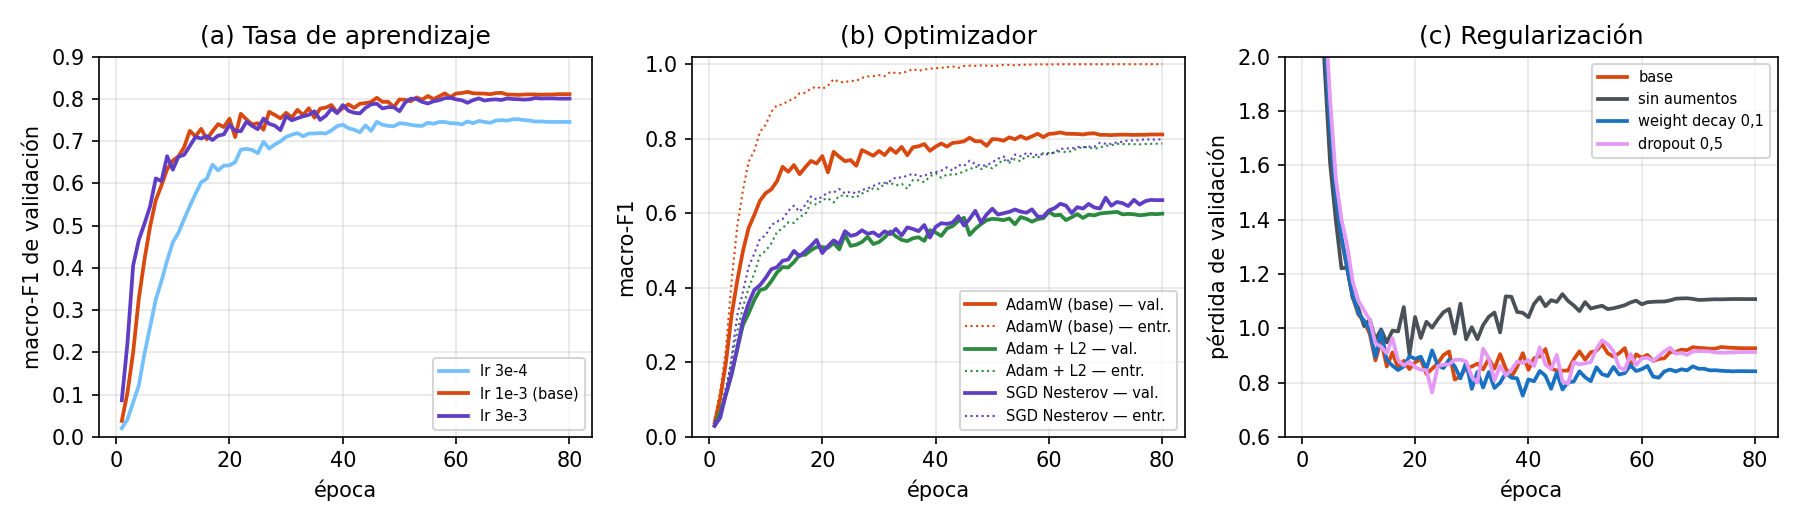
\includegraphics[width=0.86\textwidth]{figures/fig2_hiperparametros.png}
\caption{Medias de los siete folds. (a) Macro-F1 de validación según la tasa de aprendizaje; (b) macro-F1 de entrenamiento (punteado) y de validación según el optimizador; (c) pérdida de validación con distintas regularizaciones.}\label{fig:hiper}
\end{figure}

En la Figura~\ref{fig:hiper}a, con $3\times10^{-4}$ la curva sube más despacio y se estabiliza en 0,75, mientras que $10^{-3}$ y $3\times10^{-3}$ se superponen desde la época 30, así que la tasa base está en una zona estable. En la Figura~\ref{fig:hiper}b, Adam y SGD no se sobreajustan, sino lo contrario: su macro-F1 de entrenamiento se queda en 0,79 a 0,80 en la época 80, cuando AdamW ya está en 1,0; es un subajuste, que se corregiría reajustando la tasa o con más épocas, y no con más regularización. En la Figura~\ref{fig:hiper}c, sin aumentación la pérdida de validación sube desde la época 19 hasta 1,11, la señal de sobreajuste más clara; un weight decay de 0,1, en cambio, la deja en 0,84 en lugar de 0,93, es decir, mejora la calibración aunque el macro-F1 casi no cambie.

%--------------------------------------------------------------------------------------
\section{Curvas de aprendizaje y diagnóstico del modelo base}

\begin{figure}[htbp]
\centering
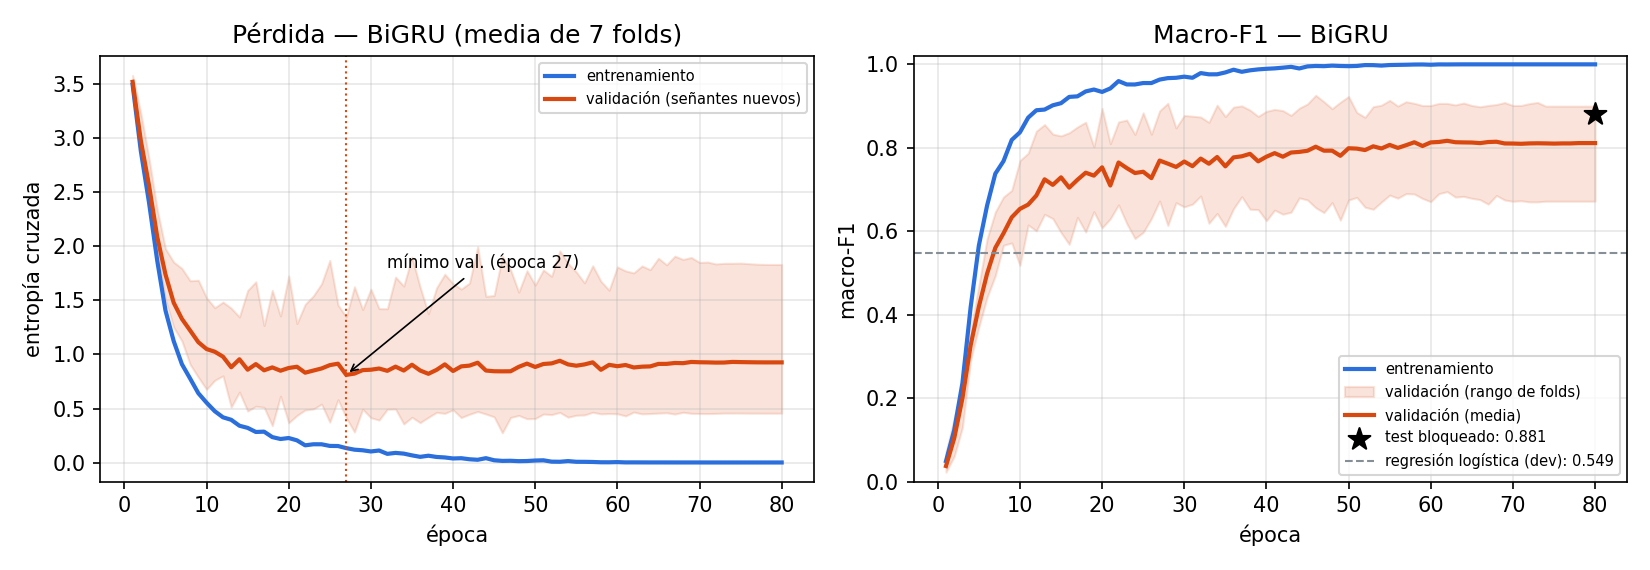
\includegraphics[width=0.68\textwidth]{figures/fig3_curvas_base.png}
\caption{BiGRU base: pérdida y macro-F1 de entrenamiento y validación por época (media de 7 folds; la franja es el rango entre folds). La estrella marca el resultado del test bloqueado, que no influyó en ninguna decisión.}\label{fig:curvas}
\end{figure}

En la Figura~\ref{fig:curvas}, el macro-F1 de entrenamiento llega a 1,0 hacia la época 40 y el de validación se estabiliza en 0,81 sin caer: la red memoriza a los doce señantes de entrenamiento de cada fold, pero esa memorización no destruye lo que generaliza. La pérdida de validación, en cambio, toca su mínimo en la época 27 (0,81) y luego sube hasta 0,93, lo que se interpreta como un sobreajuste de confianza más que de decisión: la red se vuelve más segura de sus predicciones, también de las equivocadas, y la entropía cruzada lo castiga aunque los aciertos sigan aumentando. Por esto, una parada temprana por pérdida habría cortado demasiado pronto, ya que las mejores épocas por macro-F1 van de la 40 a la 78. La franja entre folds es ancha (de 0,67 a 0,90 al final), señal de que la persona evaluada pesa más que cualquier hiperparámetro; el test (0,881) cae en la parte alta de ese rango, en coherencia con la mejor detección de sus señantes.

%--------------------------------------------------------------------------------------
\section{Resultados y comparación con la línea base}

Antes de abrir el test se registró la decisión (\code{reports/e3\_final/DECISION.md}): evaluar la BiGRU base sin las variantes de la Tabla~\ref{tab:experimentos}, porque ninguna la supera de forma distinguible del ruido y escoger la mejor de 14 opciones evaluadas en los mismos folds habría inflado la estimación. Luego ambos modelos se entrenaron con los catorce señantes de desarrollo y se evaluaron una sola vez sobre los cuatro del test (Tabla~\ref{tab:resultados}).

En desarrollo, la BiGRU mejora el macro-F1 en 0,263 en promedio y gana en los siete folds (Figura~\ref{fig:comparacion}a); sobre las predicciones agrupadas la mejora es de 0,244, y el remuestreo de señantes, con 2.000 réplicas, da un intervalo del 95\,\% de +0,16 a +0,37 (Tabla~\ref{tab:resultados}), y frente a la variante de la línea base con filtro de plausibilidad la ventaja es similar (+0,251; [+0,16; +0,35]), de modo que la regla del plan se cumple con amplitud. La mejora no es pareja: es muy grande en el fold 3, el del señante S2-19 (de 0,20 a 0,84), y menor en el fold 7 (+0,10). Ninguna de las 43 clases empeora; los números pasan de un F1 medio de 0,43 a 0,71 y la cortesía, de 0,61 a 0,85. Las mayores ganancias están en «baño» (+0,57), «excelente» (+0,49), «hola» y «dos» (+0,38), señas que se distinguen más por la trayectoria de la mano que por su posición promedio.
En el test la ventaja se confirma en los cuatro señantes (Figura~\ref{fig:comparacion}b) y es mayor donde la línea base fallaba: S2-01 pasa de 0,55 a 0,90 y S2-31, de 0,37 a 0,69. Ambos modelos obtienen más en test porque sus señantes tienen mejor detección; por eso pesa más la diferencia entre modelos (+0,20 en test y +0,26 en desarrollo) que los valores absolutos. Con cuatro personas el intervalo por señantes es amplio, de +0,09 a +0,35 (de +0,16 a +0,25 si se remuestrean videos), pero queda lejos de cero.

\begin{table}[htbp]
\centering
\caption{Desempeño en desarrollo y en el test bloqueado. Última fila: diferencia de macro-F1 (en desarrollo, media de folds) e IC del 95\,\% por señantes.}\label{tab:resultados}
\small
\setlength{\tabcolsep}{4pt}
\renewcommand{\arraystretch}{1.1}
\begin{tabularx}{\textwidth}{@{}>{\raggedright\arraybackslash}p{3.0cm}>{\centering\arraybackslash}p{2.5cm}*{3}{>{\centering\arraybackslash}X}>{\centering\arraybackslash}p{2.5cm}*{2}{>{\centering\arraybackslash}X}@{}}
\toprule
& \multicolumn{4}{c}{\textbf{Desarrollo (7 folds)}} & \multicolumn{3}{c}{\textbf{Test bloqueado}}\\
\cmidrule(lr){2-5}\cmidrule(l){6-8}
\textbf{Modelo} & \textbf{Macro-F1} & \textbf{Exactitud} & \textbf{Top-3} & \textbf{Peor señante} & \textbf{Macro-F1} & \textbf{Exactitud} & \textbf{Top-3}\\
\midrule
Regresión logística & 0,548 $\pm$ 0,166 & 0,569 & 0,783 & 0,11 & 0,685 & 0,669 & 0,829\\
\textbf{BiGRU base} & \textbf{0,811 $\pm$ 0,079} & \textbf{0,811} & \textbf{0,923} & \textbf{0,53} & \textbf{0,881} & \textbf{0,869} & \textbf{0,955}\\
\midrule
Diferencia (IC) & +0,263 [+0,16; +0,37] & \multicolumn{3}{c}{mejora en 7 de 7 folds} & +0,196 [+0,09; +0,35] & \multicolumn{2}{c}{en 4 de 4 señantes}\\
\bottomrule
\end{tabularx}
\end{table}

\begin{figure}[htbp]
\centering
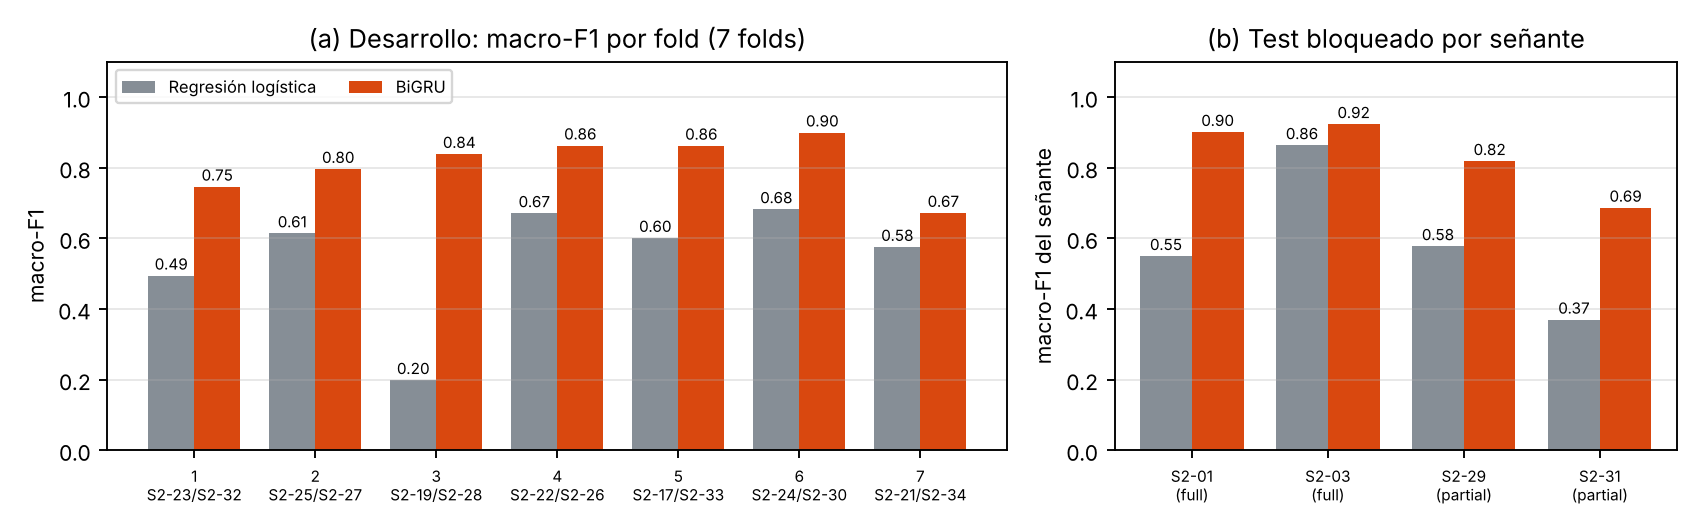
\includegraphics[width=0.68\textwidth]{figures/fig4_comparacion.png}
\caption{(a) Macro-F1 por fold en desarrollo, con los dos señantes de cada fold; (b) macro-F1 por señante en el test bloqueado.}\label{fig:comparacion}
\end{figure}

En costo, la BiGRU tarda unos 183 s por fold en CPU, frente a 1,8 s de la regresión logística, y predice un video en 3 a 7 ms, cifra menor frente a los 2,5 s por video de MediaPipe. La convolución temporal es la red más barata (154 s por fold y 0,7 ms por video), con un desempeño que no se distingue del de la BiGRU.

%--------------------------------------------------------------------------------------
\section{Análisis de errores}

Los errores de la BiGRU no se reparten al azar. El primer grupo son números que comparten la forma de la mano: en desarrollo predominan seis $\rightarrow$ uno (12 videos), siete $\rightarrow$ dos (12) y uno $\rightarrow$ seis (10), y en el test la mitad de los «seis» se clasifican como «uno» (Figura~\ref{fig:errores}b). Estas señas se distinguen por qué dedos se extienden, un detalle que 21 puntos por mano en dos dimensiones parecen no resolver bien. El segundo grupo son «sí» (F1 = 0,50), «necesitar» (0,52) y «no» (0,55), las más difíciles; una hipótesis razonable es que parte de su información está en la cabeza o en la expresión facial, que se dejaron fuera por privacidad y parsimonia, pues de la cabeza solo se conserva la nariz.

\begin{figure}[htbp]
\centering
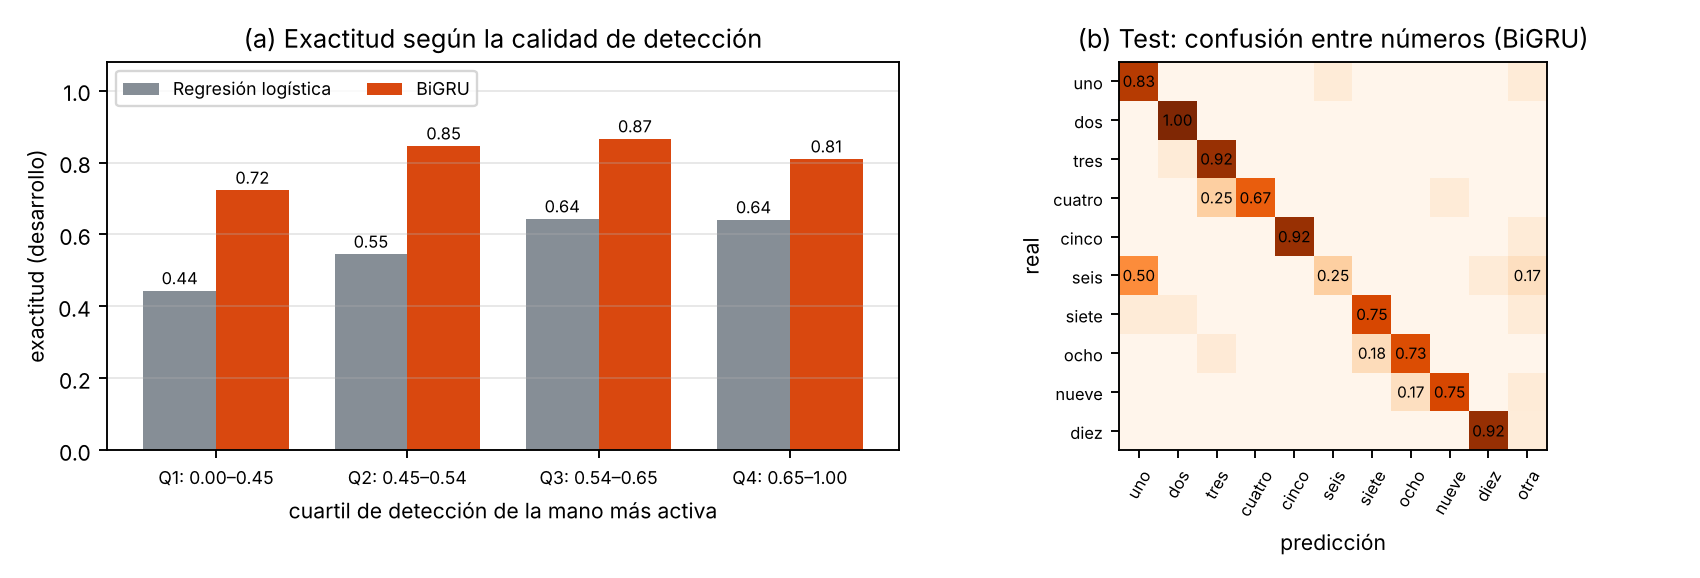
\includegraphics[width=0.68\textwidth]{figures/fig5_errores.png}
\caption{(a) Exactitud por video según el cuartil de detección de la mano más activa, en desarrollo; (b) matriz de confusión de la BiGRU entre los números en el test, normalizada por fila.}\label{fig:errores}
\end{figure}

El tercer factor es la detección (Figura~\ref{fig:errores}a). Por video, la BiGRU acierta el 72\,\% en el cuartil con peor detección y entre el 81\,\% y el 87\,\% en los demás, mientras que la regresión logística pasa del 44\,\% al 64\,\%. Por señante, en cambio, la detección media no explica de forma significativa el desempeño de ninguno de los modelos con catorce personas (Spearman de $-$0,40, $p$ = 0,15, para la BiGRU y de 0,25, $p$ = 0,39, para la regresión logística). El caso de S2-19 resume el patrón: con detección de 0,46, pasa de 0,11 a 0,87. Leer la secuencia con una máscara parece tolerar mejor los cuadros perdidos que un resumen estadístico.

Dos señantes siguen por debajo del resto, S2-21 en desarrollo (0,53) y S2-31 en test (0,69), sin que la detección lo explique; sin metadatos de los participantes no es posible atribuirlo a la forma de señar, a la cámara o a la iluminación. Cuando la BiGRU se equivoca, la seña correcta está entre sus tres primeras opciones en el 59\,\% de los casos.

%--------------------------------------------------------------------------------------
\section{Oportunidades de mejora, limitaciones y conclusiones}

Leer la secuencia completa supera con claridad a resumirla en estadísticas: la BiGRU sube el macro-F1 de 0,548 a 0,811 en desarrollo y de 0,685 a 0,881 en el test, gana con todas las personas evaluadas y reduce a la mitad la variación entre ellas. La aumentación, la máscara y la duración aportan; la tasa de $10^{-3}$ está en una zona estable; y, con la tasa y la regularización de la base sin reajustar, Adam y SGD no convergen en 80 épocas. Se derivan cinco caminos de mejora:

\begin{itemize}
\item \textbf{Codificador convolucional.} La Conv1D empata con la GRU con una cuarta parte del costo de inferencia, de modo que la ganancia proviene de modelar la secuencia y no de la recurrencia en sí, y sería la candidata para tiempo real.
\item \textbf{Combinar los ajustes neutros.} Un weight decay de 0,1 y quitar la interpolación podrían probarse juntos en una segunda ronda, lo que no se hizo antes del test para no seleccionar entre más variantes.
\item \textbf{Forma de la mano y cabeza.} Ángulos entre falanges, distancias entre puntas de dedos o la profundidad que entrega MediaPipe podrían separar los números; para «sí» y «no», puntos de la cabeza.
\item \textbf{Calibración.} La subida de la pérdida de validación indica exceso de confianza; un escalado de temperatura sería un ajuste barato antes de mostrar probabilidades a un estudiante.
\item \textbf{Más personas.} La mayor fuente de variación es el señante, de modo que más señantes, y más diversos, ayudarían más que cualquier hiperparámetro.
\end{itemize}

En cuanto a las limitaciones, (1) catorce señantes de desarrollo y cuatro de test dejan intervalos amplios, y los resultados valen para este grupo, del que no hay datos demográficos; (2) se usó una semilla por fold, así que la dispersión refleja a las personas y no la variación del entrenamiento; (3) los optimizadores alternativos no se evaluaron con su propia tasa; (4) 43 señas aisladas no permiten hablar de la lengua en uso; y (5) el test tiene mejor detección que desarrollo, por lo que sus valores absolutos son algo optimistas. Por ello, el modelo sirve como base para una herramienta de práctica, no como traductor ni como reemplazo de un intérprete, y cualquier uso real exige validarlo con la comunidad sorda y con docentes de LSC. Todo se reproduce con \mbox{\code{pytest -q}}, \code{scripts/run\_experiments.py} y \code{scripts/compare\_models.py}; en Linux, la BiGRU base dio 0,808 $\pm$ 0,079 frente a 0,811.

%--------------------------------------------------------------------------------------
\section*{Referencias}
\sloppy\footnotesize
\setlength{\parskip}{2pt}
\noindent\hangindent=1.2em Cho, K., van Merriënboer, B., Gulcehre, C., Bahdanau, D., Bougares, F., Schwenk, H., y Bengio, Y. (2014). Learning phrase representations using RNN encoder-decoder for statistical machine translation. \emph{arXiv:1406.1078}.\par
\noindent\hangindent=1.2em Google Developers. (s.~f.). A scientific approach to improving model performance. \url{https://developers.google.com/machine-learning/guides/deep-learning-tuning-playbook/scientific}\par
\noindent\hangindent=1.2em Hochreiter, S., y Schmidhuber, J. (1997). Long short-term memory. \emph{Neural Computation, 9}(8), 1735-1780.\par
\noindent\hangindent=1.2em Loshchilov, I., y Hutter, F. (2019). Decoupled weight decay regularization. En \emph{International Conference on Learning Representations (ICLR)}.\par
\noindent\hangindent=1.2em Lugaresi, C., et al. (2019). MediaPipe: A framework for building perception pipelines. \emph{arXiv:1906.08172}.\par
\noindent\hangindent=1.2em MLflow Project. (s.~f.). MLflow Tracking. \url{https://mlflow.org/docs/latest/ml/tracking/}\par
\noindent\hangindent=1.2em Mora-Zarate, J. E., Garzón-Castro, C. L., y Castellanos-Rivillas, J. A. (2025). LSC-54: A landmark-based dataset for Colombian Sign Language. \emph{Data in Brief, 63}, 112145. \url{https://doi.org/10.1016/j.dib.2025.112145}\par

\end{document}
